\documentclass[a4paper]{scrartcl}
\usepackage[cm]{fullpage}
\usepackage{amsmath, amssymb, esint}
\usepackage{siunitx}
\usepackage[backend = biber, style = numeric-comp]{biblatex}

\usepackage{tikz}

\begin{filecontents}{\jobname.bib}
@misc{wiki:pendulum,
    author = "Wikipedia",
    title = "Pendulum (mathematics) --- Wikipedia{,} The Free Encyclopedia",
    year = "2016",
    url = "https://en.wikipedia.org/w/index.php?title=Pendulum_(mathematics)&oldid=714064721",
    note = "[Online; accessed 16-May-2016]"
}
@misc{BGI2016,
    url = {http://bgi.omp.obs-mip.fr/data-products/Toolbox/Prediction-of-gravity-value},
    year  = {2016},
    month = {apr},
    title = {Prediction of gravity value},
    author = {The International Gravimetric Bureau ({BGI})},
    howpublished = {Online tool}
}
\end{filecontents}
\addbibresource{\jobname.bib}

\begin{document}

\title{PHYS2113: Kater's Pendulum}
\author{ \\ \\}
\date{2016-05-11}
\maketitle

\begin{abstract}
    A Kater's pendulum was used to measure the effective gravity at the UNSW Kensington second year physics lab (33.918 S 151.2303 E to within \SI{20}{\metre}, with an altitude of \SI{50 \pm 10}{\metre} on the WGS84 datum), and was found to be \SI{9.82 \pm 0.04}{\metre\per\second\squared}. This corresponds to a real gravity of \SI{9.84 \pm 0.04}{\metre\per\second\squared}.
\end{abstract}

\section{Introduction}
Please refer to the student notes of the experiment.

\section{Materials and Methods}
Please refer to the operating instructions and prework of the experiment.

A run-of-the-mill 30 fps HD camera, a 15 fps \(800 \times 448\) px webcam, and the known-to-be-inaccurate stopwatch \#6 were used for measuring the period.

The pendulum was started with initial angle less than \(\frac{\pi}{20} \:\si{\radian} = \SI{9}{\degree}\) in either direction, to allow the \(\sin x \approx x\) approximation to hold, and timed for about a minute each.

Comparing the small angle approximated solution to the non-approximated solution \(T_{unapprox} = \frac{2 T}{\pi} K(\sin^2 \frac{\theta_0}{2})\), where \(T\) is the period of the small angle approximation and \(K\) the complete elliptic integral of the first kind \cite{wiki:pendulum}, we find that \(T \approx 0.9985 T_{unapprox}\) for \(\theta_0 = \frac{\pi}{20}\).

Pushing this value through our equation for \(g\) yields \(g = \frac{4 K(\sin^2 \frac{\theta_0}{2})^2}{\pi^2} g_{unapprox} \approx 1.0031 g_{unapprox}\), where \(g_{unapprox}\) is the \(g\)-value that would have been gotten with the raw uncorrected \(T_{unapprox}\).

\section{Results}
\begin{table}[d]
    \centering
    \begin{tabular}{c | c | c}
        & Stopwatch Measurement & Camera Measurement \\
        \hline
        \(T_1\) (\si{\second}) & \SI{1.95 \pm 0.01}{} & \SI{1.999 \pm 0.002}{} \\
        \(T_2\) (\si{\second}) & \SI{1.95 \pm 0.01}{} & \SI{1.999 \pm 0.001}{} \\
        \hline
        \(g_{unapprox}\) (\si{\metre\per\second\squared}) & \SI{10.3 \pm 0.1}{} & \SI{9.79 \pm 0.02}{} \\
        \(g\) (\si{\metre\per\second\squared}) & \SI{10.3 \pm 0.2}{} & \SI{9.82 \pm 0.04}{} \\
        \(g_{real}\) (\si{\metre\per\second\squared}) & \SI{10.3 \pm 0.2}{} & \SI{9.84 \pm 0.04}{}
    \end{tabular}
    \caption{Period measurements and corresponding \(g\)-values}
    \label{tab:periods}
\end{table}

\begin{table}[d]
    \centering
    \begin{tabular}{c | c}
        Variable & Error Contribution (\si{\milli\metre\per\second\squared}) \\
        \hline
        \(L\) & \SI{10}{} \\
        \(l_1\) & \SI{0}{} \\
        \(T_1\) & \SI{7}{} \\
        \(T_2\) & \SI{13}{} \\
        \(\theta_0\) & \SI{40}{}
    \end{tabular}
    \caption{Error breakdown for the camera-measured \(g\)}
    \label{tab:errors}
\end{table}

\begin{figure}[d]
    \centering
    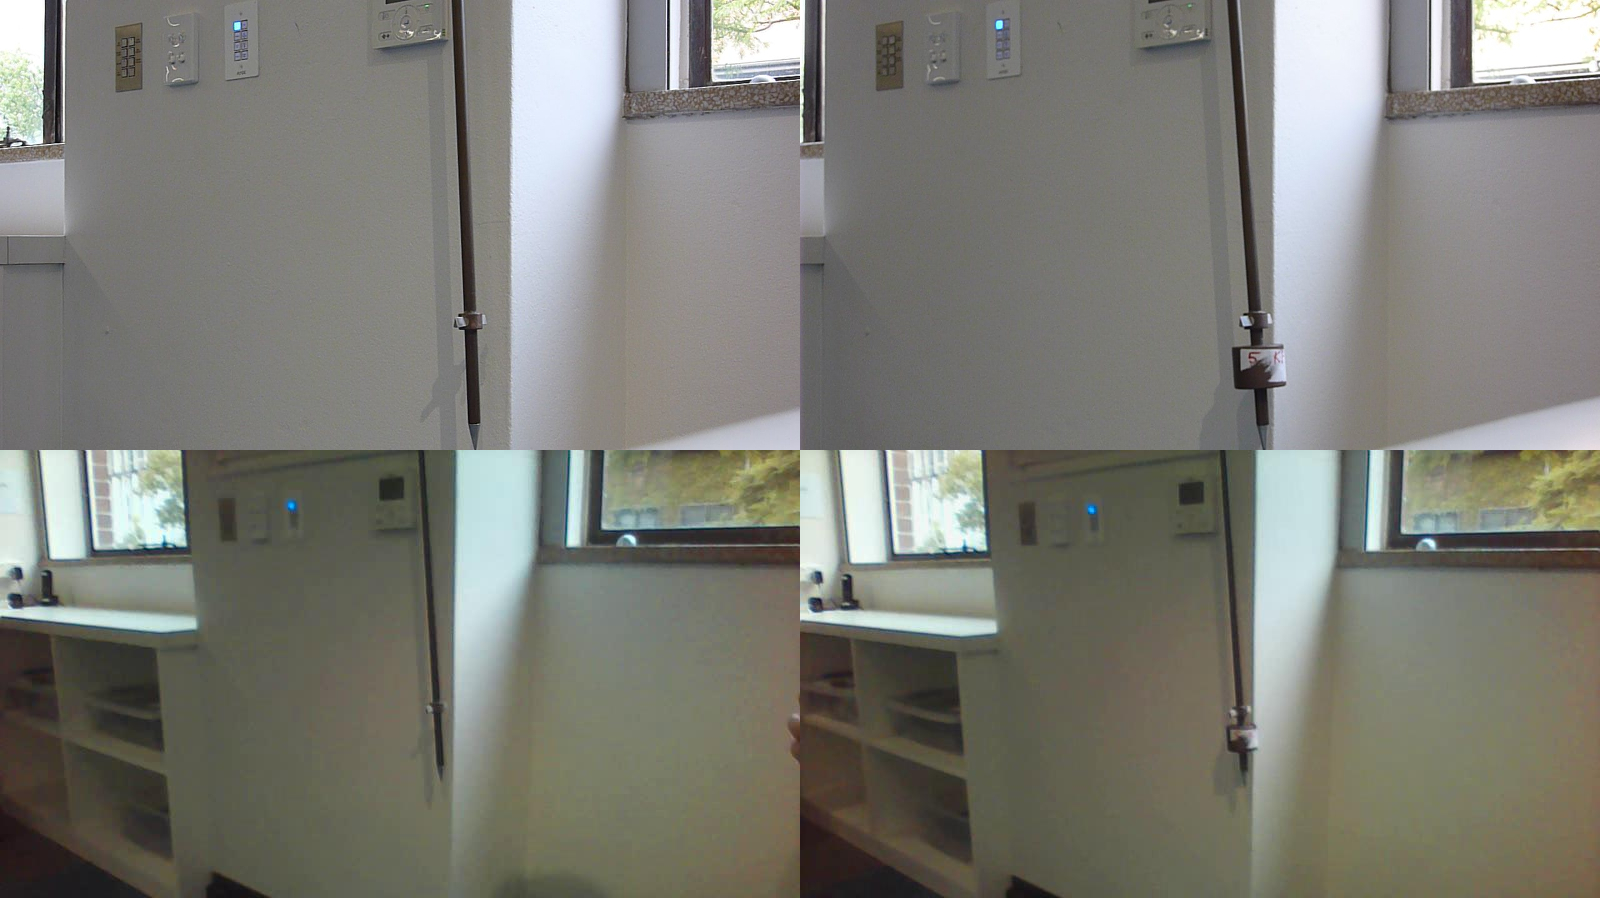
\includegraphics[width = 18cm]{video.jpg}
    \caption{Pendulum peaks. Left: \(T_1\); Right: \(T_2\); Top: HD Camera; Bottom: Webcam}
    \label{fig:video}
\end{figure}

Both GPS and Google map measurements showed that the experiment took place at 33.918 S 151.2303 E to within \SI{20}{\metre}, with an altitude of \SI{50 \pm 10}{\metre}. This corresponds to an interpolated \(g = \SI{9.797}{\metre\per\second\squared}\) from other measurements \cite{BGI2016}, or \(g = \SI{9.799}{\metre\per\second\squared}\) with the formula provided in the student notes.

This is approximately \SI{5298}{\kilo\metre} from the rotation axis of the Earth (with the WGS84 datum) and corresponds to a centrifugal force of \SI{0.02817}{\metre\per\second\squared} directed north with \SI{56.082}{\degree} of elevation. This is used to calculate \(g_{real}\).

The period of the pendulum was measured when it was swinging north-to-south, so the coriolis force would be negligible.

The pivot-to-pivot distance \(L\) was measured to be \SI{991 \pm 1}{\milli\metre}, while the \(l_1\) distance (as defined in the prework) was measured to be \SI{199 \pm 1}{\milli\metre}.

While a protractor was unavailable to measure angles, eyeballing the pendulum seemed to show that our starting angle \(\theta_0\) was \(\frac{\pi}{20} \pm \frac{\pi}{30} \:\si{\radian}\).

The measured pendulum periods are shown in Table \ref{tab:periods}, as well as the corresponding \(g\)-values, while Table \ref{tab:errors} shows the individual errors contributing to the final error estimate of the camera-measured \(g\). Figure \ref{fig:video} shows the initial peak position of the pendulum for the different measurements.

The stopwatch was also recorded with the 15 fps camera, and was found to run \SI{101.6 \pm 0.1}{\percent} the speed of the camera.

\section{Discussion}
The \(g\) value obtained by the stopwatch measurement is clearly absurd, since it is well known that the surface gravity of earth does not vary more than \SI{1}{\percent} from \SI{9.8}{\metre\per\second\squared}. This was expected, since it was known that the stopwatch was inaccurate. In fact, recording the stopwatch from a 15 fps webcam (which is calibrated to the highly accurate computer clock) indicated it was running fast, hence giving a smaller period and larger gravity measurement.

However, the \(g\) value obtained by camera is much more reasonable, where the reference values are within error, while the centre value is within \SI{0.3}{\percent} of the reference values. This result will be used for the following discussion.

From the errors taken into account for the calculations, the main contributor of error was the uncertainty in initial pendulum angle \(\theta_0\). This could be significantly lowered by having a fixed starting angle by way of a peg stuck in the wall near the bottom of the pendulum, and starting the pendulum from where it just touches the peg each time.

Next is the error in \(T_2\). This (along with the error in \(T_1\)) can be reduced simply by averaging the period over more oscillations of the pendulum, since the error is inversely proportional to the number of swings. One could use a higher frame rate camera (for better temporal resolution), as well as moving it closer (for better spatial resolution) to avoid the issue of having multiple consecutive frames with the same perceived pendulum position. Alternatively, an instrument that can electronically measure the angular displacement could be used, which would provide much better temporal and spatial resolution than a camera.

The error in \(L\) can not be improved much further with a ruler alone, since it approaches the precision of the ruler. One would have to use a different and more precise instrument, such as a laser rangefinder, to reduce the error significantly.

Unaccounted for errors could include the effects of air, such as drag, currents and buoyancy. This would increase the measured period and thus the calculated \(g\) would be below the real value. Performing the experiment in a vacuum would eliminate this error.

Other unaccounted for errors could be associated with the pivot, such as frictional losses and a non-point pivot. Friction would also increase the measured period, while it is unknown what effect a non-point pivot would have. This error could be reduced by lubricating the pivot well, as well as ensuring the pivots are at a perfect right angle to the pendulum and are as thin as possible.

\printbibliography

\end{document}